%%
%% Author: darshan
%% 08/03/18
%%

% Preamble
\documentclass[11pt]{report}

% Packages
\usepackage{a4wide}

% Document
\begin{document}
    \chapter{Approach / Implementation}




    \section{Theoretical Basics and Concept}




    \section{Implementation Overview}




    \section{Pipeline Implementation}




    \section{Provenance API}




    \section{Cassandra as Provenance DB}




    \section{User Interface}

    Today most IS systems are based upon a Client-Server architecture, a three-tiered approach. The server performs the grunt of all operations where as the client side is more concerned with how to present the data. The processes that go on in these tiers can be represented by many more tiers, for instance a database tier can be added, where all data is stored can be represented by the diagram below. However it is important to note that more than one tier can be stored on one server, for instance both the web server and database servers each represent there own tiers in the diagram below, but in reality they could be seen as one.

    To  implement  a  web  application for Error detecting and monitoring system, client-server  architecture  is  required.  The  most  popular  client-server architectures  are  the  two-tier  and  the  three-tier architecture. The choice   of   architecture   affects   the   development   time   and   the   future   flexibility   and maintenance  of  the  application.  While  selecting the  architecture  most  suitable  for  an  application, many  factors  including  the complexity  of  the  application,  the  number  of  users and their geographical dispersion are considered. This system  is designed  based  on  a  traditional  three-tier  architecture  used  by  many  web  applications. Three-tier architecture  includes  a  presentation layer,  business  rules/  logic  layer, and the data layer (provenance database). The three-tier architecture is shown in Figure \ref{fig:architecture}.

    \begin{figure}
        \centering
        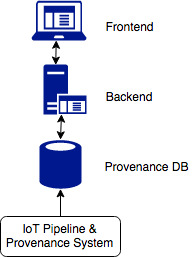
\includegraphics[width=0.4\textwidth]{figures/architecture.jpg}
        \caption{\label{fig:architecture}This is three-tier architecture.}
    \end{figure}

    Three-tier architecture gives an enhanced security, through the implementation of several layers, enhances the data security on a service-by-service. As client do not interact with the database directly, it provides less risk and confliction with unauthorized data. Also it improves the data integrity as data corruption through client application can be eliminated as the data is passed in the middle tier for database updations ensures its validity. Due to distributed deployment of application servers, scalability of the system is enhances since a separate connection from each client is not required whereas connections from few applications servers are sufficient.
    \newline
    \newline
    The three-tier architecture is generally used when an effective   distributed client/server design is needed that provides
    \begin{itemize}
        \item increased performance
        \item flexibility
        \item maintainability
        \item reusability and
        \item scalability
    \end{itemize}

    This  model hides  the  complexity  of  distributed  processing  from  the  user.  These features   have   made   the   three-tier   architecture   a   popular choice over the two-tier architecture for Internet applications. The three layers are discussed below.
    \newline
    \newline
    The \textbf{Data layer} is  responsible  for  data  storage.  Primarily  this  tier  (layer)  consists of one or more relational databases and/or file systems.
    \newline
    \newline
    The \textbf{Business Rules/Logic layer} is the middleman between the presentation layer and  the  data  layer. This  middle  tier  was  introduced  to  overcome  the  deployment limitation (whenever
    the application logic changed the application had to be redistributed at  each  and  every  client)  in  the  two-tier  architecture.  The  middle  tier  provides  process
    management where business logic and rules are executed and can accommodate hundreds of  users.
    \newline
    \newline
    The \textbf{Presentation  Layer},  also  called  the Client  tier,  is responsible  for the presentation  of  data,  receiving  user  events,  and  controlling  the  user  interface.  The  user
    interaction with the system is entirely through this layer.
    \newline
    \newline
    The three-tier architecture for Smart-grid IoT provenance system's Error detection use-case. The data layer in this architecture comprises of Provenance Database of the system, in this case here we have used Cassandra. The logic layer/business layer is defined by Java's Spring boot framework and provides REST component to the Presentation layer and the messages are communicated by JSON. And the Presentation layer where the data is represented to the end-user is developed in Node.js Express framework with Jade view template engine.

    In the next section, there is a detail description for Backend and Frontend.



    \subsection{Backend}




    \subsection{Frontend}


    \section{Testing and Deployment}


\end{document}